\chapter{Una torre más o menos medieval -- I}

\lettrine[lines=2]{C}{uando Cecilia} entró al día siguiente en la
oficina de Antonia, la encontró frente a un nuevo objeto en el monitor
de la computadora.


\begin{figure}[ht]
  \centering
  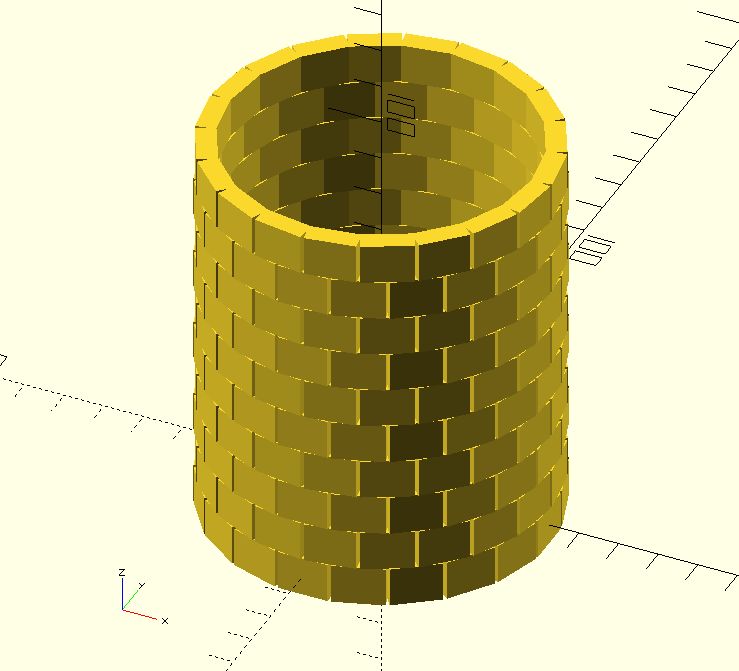
\includegraphics[width=.55\textwidth]{imagenes/torre-tentativa}  
  \caption{Una torre más o menos medieval.}
  \label{fig:torre-tentativa}
\end{figure}



---¿Con qué estás jugando ahora, Antonia? ---preguntó con una sonrisa,
mientras se sentaba a su lado.

---Quería introducirte un nuevo concepto, que considero fundamental a
esta altura del manual ---empezó Antonia, para asombro de Cecilia que
nunca supo que estaba participando de un ``manual''---. Hasta ahora
estuvimos escribiendo a partir de los objetos primitivos que
\openscad{} nos ofrece; sin embargo, el lenguaje también nos brinda la
posibilidad de crear nuestros propios objetos `básicos' (y no tan
básicos), a fin de usarlos como cualquier otro en nuestra descripción
de una escena.

Cecilia sintió de golpe que siempre supo, en el fondo, que esa
posibilidad \emph{debía} existir.

---Para mostrarte cómo se concreta esa posibilidad, se me ocurrió que
podemos crear algo como esto ---continuó Antonia señalando el monitor
con el mentón---: Una torre que evoca recuerdos más o menos
medievales. Mi idea es que la construyamos en tres pasos, definiendo
para ello tres nuevos `objetos', que dependerán cada uno del anterior:
el objeto `ladrillo', el objeto `piso' y el objeto `torre'. Es decir,
vamos a escribir la torre como un objeto hecho de `pisos', y cada piso
como un objeto hecho de `ladrillos'.\footnote{El improbable lector de
  este librito no debe dejarse confundir con el uso impreciso e
  informal que hace Antonia del témino ``objeto'' en un contexto
  computacional: los objetos a los que hace referencia nada tienen que
  ver con los que pueblan lenguajes como Smalltak, C++ o Java, entre
  otros. (Nota del Editor)}

\section{Módulos}


\guillemotright La manera de crear la definición de un objeto es con
la palabra \lstinline!module!.

\subsection{El ladrillo}

\begin{figure}[ht]
  \begin{minipage}[]{.6\textwidth}
    \begin{lstlisting}
module ladrillo(size) {
  cube(size, center=true);
}
    \end{lstlisting}
  \end{minipage}\hfill
    \begin{minipage}[]{.4\textwidth}
      \centering
      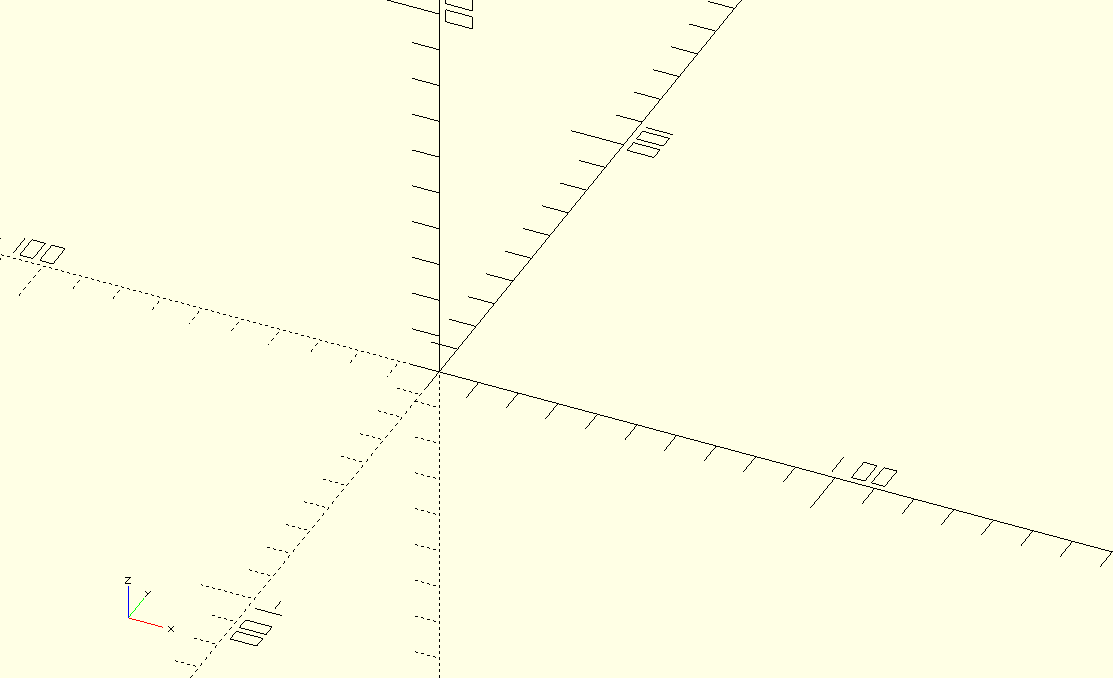
\includegraphics[width=.9\textwidth]{imagenes/vacio}
    \end{minipage}
    \caption{Antonia define el módulo \texttt{ladrillo}.}
    \label{fig:modulo-ladrillo}
  \end{figure}
  
  Cecilia sintió la incómoda sensación de que Antonia se estaba
  burlando de ella: ¡La pantalla aparecía vacía! Si bien no dijo nada,
  su expresión debió haber sido lo suficientemente elocuente como para
  que hasta Antonia se diera cuenta:

  ---Es natural que nada haya aparecido ---la tranquilizó con una
  sonrisa---; tan sólo hemos definido el objeto; aún no lo hemos
  usado.

  \guillemotright La palabra \lstinline!module! debe ir seguida por el
  nombre que queremos darle al nuevo objeto. Inmediatamente después
  deben ir, entre paréntesis, los parámetros que determinarán el
  mismo: en nuestro caso, su tamaño\footnote{Nos hubiera encantado
    usar la palabra ``tamaño'' en el código, pero por alguna razón
    \openscad{} se niega a aceptar variables con una ``ñ''... ¡Y nos
    negamos rotundamente a estampar la palabreja ``tamanio'', ni
    siquiera en este manualcito!}. Podría ocurrir, aunque es raro, que
  necesitemos un objeto cuya determinación sea fija e inamovible: en
  ese caso aún debemos escribir los paréntesis, sólo que estarán
  vacíos. Finalmente, escribiremos entre llaves las acciones que harán
  posible nuestro objeto: en nuestro caso, y por simplicidad, decidí
  que fuera un mero cubo, cuyo tamaño sea el parámetro de la
  definción, y esté centrado en el origen.


  Cecilia seguía en silencio y mirando el monitor; no estaba segura de
  comprender.

  Antonia prosiguió:

  ---Ahora sí podemos usar nuestro flamante ladrillo ---y escribió las
  líneas de la figura \ref{fig:codigo-ladrillo}.

  
\begin{figure}[ht]
  \begin{minipage}[]{.5\textwidth}
    \begin{lstlisting}
ladrillo([20,10,5]);
translate([25,0,0])
  ladrillo([10,8,20]);
    \end{lstlisting}
  \end{minipage}\hfill
    \begin{minipage}[]{.5\textwidth}
      \centering
      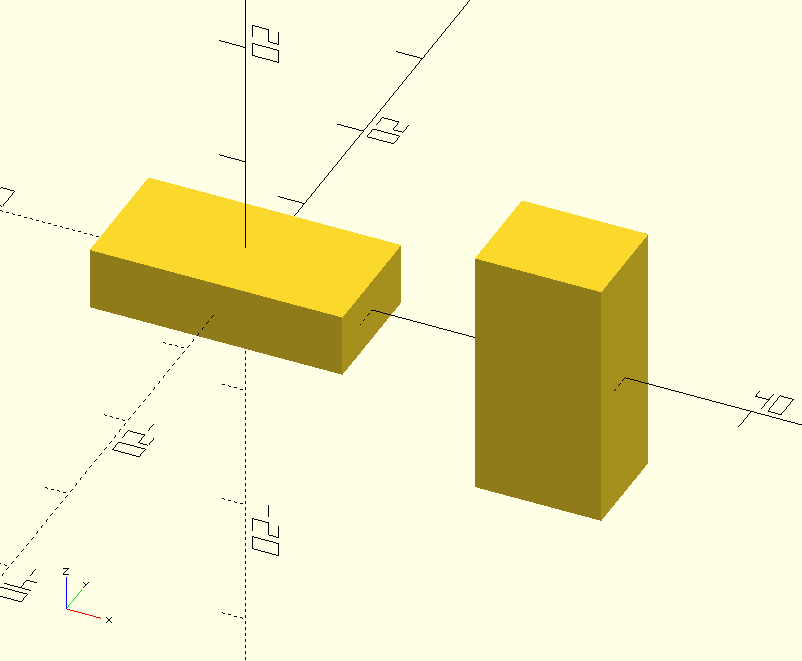
\includegraphics[width=\textwidth]{imagenes/ladrillos}
    \end{minipage}
    \caption{Antonia usa el módulo \texttt{ladrillo}}
    \label{fig:codigo-ladrillo}
  \end{figure} 
  
  Cecilia creía empezar a entender, pero algo no le cerraba:
  
  ---Antonia, ¿para qué definís un objeto que ya existe? Al final, la
  definición de ladrillo sólo hace referencia a un cubo común y
  silvestre.

  Antonia se revolvió en la silla; parecía impacientarse. Cecilia no
  supo en principio si era con ella, o consigo misma. El hecho de que
  Antonia apretara los labios, como quien busca la palabra o expresión
  justa, le hizo suponer que la impaciencia se debía a su constante
  angustia de sentir que no sabía explicarse debidamente. Ésa era una
  de las mayores preocupaciones de Antonia; preocupación a veces
  desmedida. Tal vez por eso la docencia la apasionara tanto, y tal
  vez por eso la padeciera tanto.

  ---En principio ---comenzó lentamente Antonia---, fijate que al
  menos nos salvamos de indicar `\lstinline!center=true!' en cada uso
  del ladrillo. Pero eso no es lo más importante ---Antonia volvió a
  detenerse, y suspiró---.  El caso es que nosotras ahora podemos
  dedicarnos a definir y usar los otros objetos que necesitamos (el
  piso y la torre), siempre empleando para ellos el objeto
  `ladrillo'. Para esto, es verdad, podríamos usar sin problemas el
  objeto primitivo `cubo'. Pero ahora ---Antonia se inclinó
  ligeramente hacia Cecilia, intensificando el tono de su voz---,
  imaginate que recién al final, con la torre efectivamente realizada,
  nos damos cuenta de que, no sé, sería mejor que los ladrillos
  tuvieran los bordes redondeados. O que su superficie fuera rugosa. O
  que presentaran una textura ajedrezada. ¡Qué sé yo! ---Antonia
  subrayó la idea alzando sus ojos al techo---. En ese caso (que
  descubrirás que surge muy naturalmente al escribir; hay cosas cuya
  oportunidad resulta aparente recién cuando el trabajo está muy
  avanzado) sólo deberemos cambiar la definición del módulo
  `ladrillo', y no todas las apariciones de `cube' que hubiéramos
  escrito a lo largo del texto ---concluyó Antonia, escrutando en los
  ojos de Cecilia si la explicación había sido eficaz.

  Cecilia pudo sentir un atisbo de comprensión, pero creía que sólo
  entendería cabalmente el concepto que tanto trabajo le costaba a
  Antonia trasmitir cuando lo viera realizado en un caso concreto. De
  todas formas, comprendió que eso sólo sería posible avanzando, por
  lo que decidió confiar en ella y aceptar, al menos provisoriamente,
  que era buena idea encerrar el concepto de `ladrillo' en un módulo
  propio.
  
  \subsection{El piso}

  ---Muy bien ---dijo Antonia, tomando el silencio de Cecilia como un
  permiso para seguir---; ahora ataquemos el problema del
  piso. Mientras pensamos cómo hacerlo, podemos comenzar escribiendo
  el imprescindible esqueleto de su módulo.

  

\begin{lstlisting}
module piso( ) {

}
\end{lstlisting}
  % \end{minipage}\hfill
  %   \begin{minipage}[]{.5\textwidth}
  %     \centering
  %     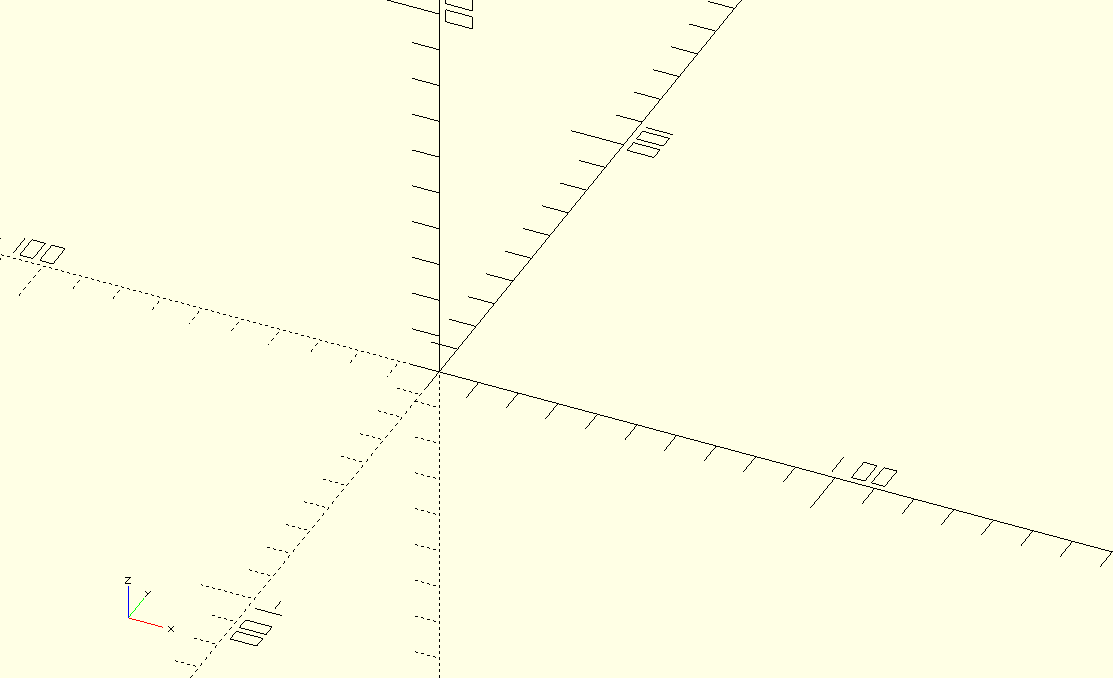
\includegraphics[width=.5\textwidth]{imagenes/vacio}
  %   \end{minipage}
  % \end{center}

  ---Pensemos ahora en los parámetros que lo definen: ¿Qué
    características determinan un piso de nuestra torre? ---y
  Antonia se detuvo, cediendo la palabra tácitamente a Cecilia, quien
  se puso a pensar en voz alta:

  ---Hmmmm.... ¿su radio?

  ---De acuerdo ---aprobó Antonia---; ¿y qué más?

  A Cecilia le empezó a gustar el juego:

  ---¿El espesor de la pared? ¿Su alto?

  ---A favor ---volvió a acordar Antonia---; ¿y qué más?

  Cecilia cerró los ojos tratando de visualizar uno de los pisos de la
  torre. Tras breves instantes, exclamó:

  ---¡La cantidad de ladrillos que lo forman!

  ---Exacto ---concluyó Antonia, y se puso a escribir:


\begin{lstlisting}
module piso(
 radio,
 altura,
 espesor,
 n_ladrillos) {
}
\end{lstlisting}
  % \end{minipage}\hfill
  %   \begin{minipage}[]{.5\textwidth}
  %     \centering
  %     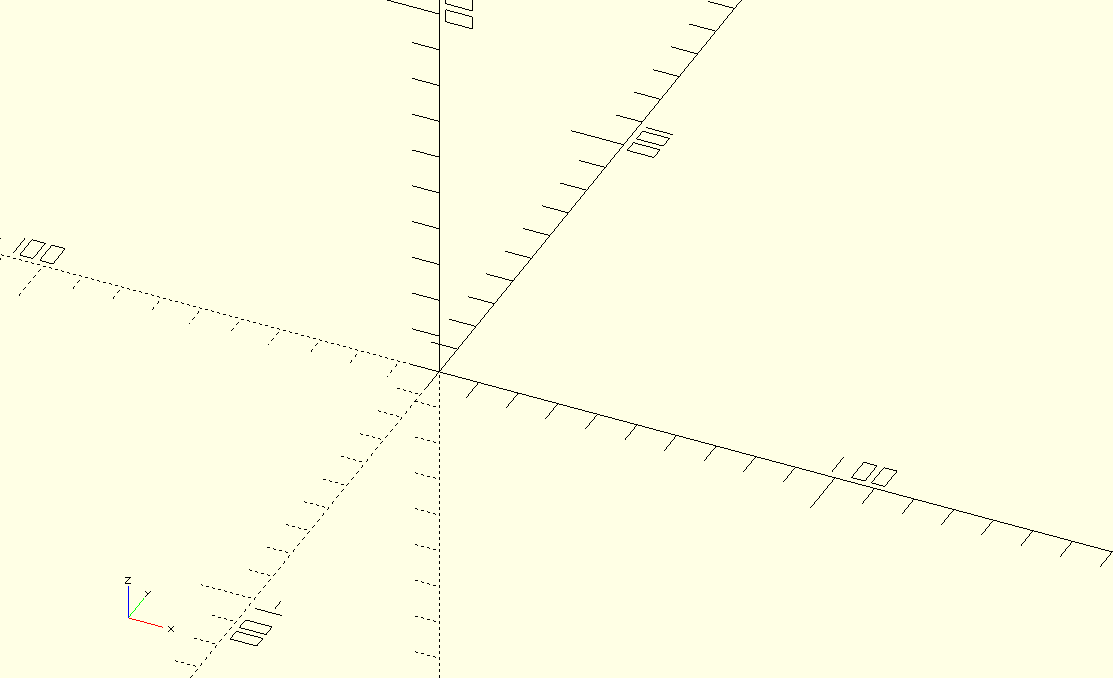
\includegraphics[width=.8\textwidth]{imagenes/vacio}
  %   \end{minipage}
  % \end{center}

---A mí, personalmente ---confesó Antonia---, y a medida que escribo
estructuras más complejas, me gusta detallar los parámetros con
nombres más elocuentes que `r', `e' o `n'. En ese caso, y para que no
me queden líneas abigarradas y difíciles de leer, escribo un parámetro
por línea. Pero es cuestión de gustos; también podrías escribir el
módulo así:

\begin{lstlisting}
//   PISO
// r: radio
// a: altura
// e: espesor
// n: cantidad de 
//    ladrillos
module piso(r,a,e,n) {
}
\end{lstlisting}
  % \end{minipage}\hfill
  %   \begin{minipage}[]{.5\textwidth}
  %     \centering
  %     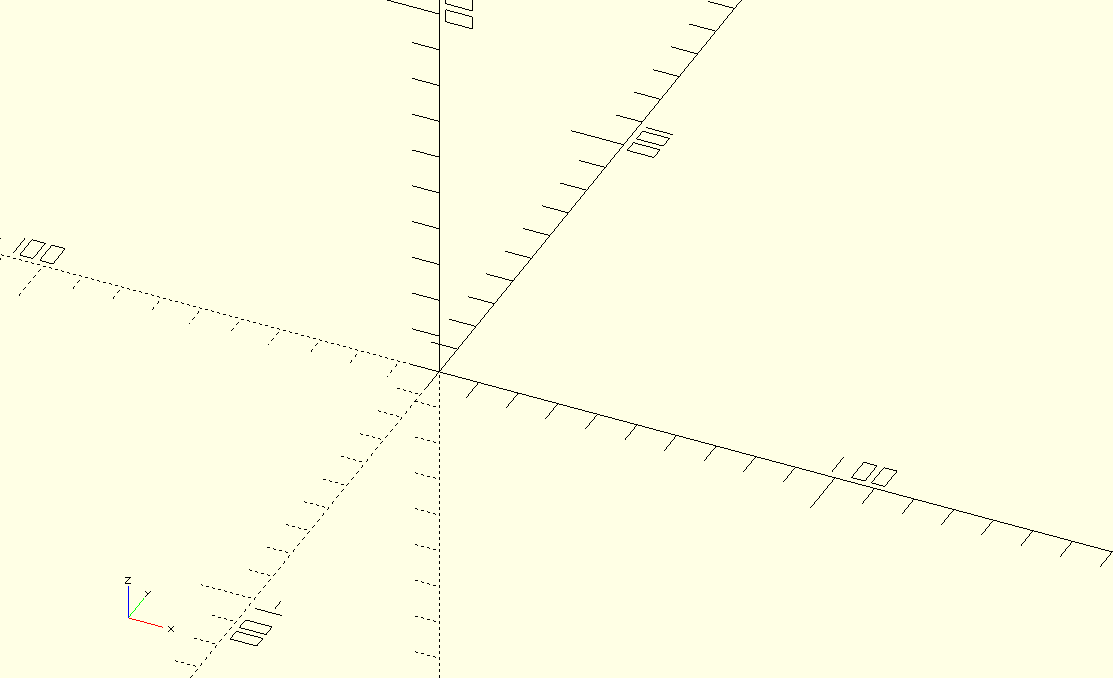
\includegraphics[width=.9\textwidth]{imagenes/vacio}
  %   \end{minipage}
  % \end{center}

Cecilia no se sentía especialmente inclinada, al menos por el momento,
hacia ninguna de las dos formas en particular.

---Ahora sí ---Antonia prosiguió---, debemos escribir, dentro de las
llaves, la forma en que efectivamente se construye un piso
---An\-to\-nia hizo una pausa, y señalando el teclado a Cecilia,
preguntó:

---¿Te animás?

Cecilia no sabía muy bien por dónde empezar, pero tomó el teclado
aparentando, lo mejor que pudo, seguridad.

<<Muy bien>> ---pensó---, <<tengo que disponer una serie de ladrillos
en círculo. ¡Pero ya hice algo parecido! Fue con esferas. No debería
ser tan distinto: crear un ladrillo, alejarlo del centro, rotarlo un
cierto ángulo, y repetir lo mismo con otros ladrillos, usando para eso
un bucle. A ver...>>

    \begin{lstlisting}
module piso(
 radio,
 altura,
 espesor,
 n_ladrillos) {
  for (alfa=[0:?:359])
   rotate([0,0,alfa])
    translate([radio,0,0])
     ladrillo([espesor,?,altura]); 
}
\end{lstlisting}
  
Cecilia, al terminar de escribir lo anterior, sintió lo que siente
todo aquél que explora un problema escribiéndolo: el sonido sordo que
produce sondear los límites de la propia comprensión del
mismo. Sintió, por un lado, que estaba bien encaminada: cada ladrillo
debía alejarse del centro una distancia igual al \texttt{radio} del
piso (línea 8), y luego rotarse un cierto ángulo \texttt{alfa} (línea
7). Además, dos de las dimensiones de cada ladrillo venían
determinadas por los parámetros de dicho piso: su \texttt{espesor} y
\texttt{altura}. Pero había dos datos cuya ignorancia sólo descubrió
al intentar describir textualmente el piso: el largo de los ladrillos,
y el ángulo que debían ser rotados. Sospechó que ambos valores
dependían del parámetro aún no empleado por ella:
\texttt{n\_ladrillos}.

Antonia parecía seguir el hilo de sus pensamientos:

---Si tuvieras que conquistar sólo una enseñanza de estos capítulos,
tal vez debería ser ésta: `Nada aclara tanto las ideas como ponerse a
escribirlas'. Y ése es quizás el mayor mérito y virtud de la
programación: obligarnos a escribir nuestras ideas con la máxima
escrupulosidad, la mayor claridad posible, la más delicada prolijidad
y una rigurosa intolerancia a cualquier forma de ambigüedad. ¡Si
supieras la cantidad de problemas que entendí mientras los escribía!
Mejor dicho: ¡gracias a que los escribía!  ---Antonia suspendió su
pequeño discurso con un tono de voz apenas exaltado. Quizá por primera
vez desde que la conocía, Cecilia no pensó que exageraba.

Volvió a sumirse en el problema: <<Bien, tengo que calcular el
incremento de \texttt{alfa} y el largo del ladrillo. El incremento es
fácil: si hay que encajar \texttt{n\_ladrillos} en una vuelta completa
de 360$^{\circ}$, dicho incremento tiene que ser igual a
$\frac{360^{\circ}}{\text{n\_ladrillos}}$. Voy a escribirlo en la
línea 6:>>


    \begin{lstlisting}
module piso(
 radio,
 altura,
 espesor,
 n_ladrillos) {
  i_alfa=360/n_ladrillos;
  for(alfa=[0:i_alfa:359])
   rotate([0,0,alfa])
    translate([radio,0,0])
     ladrillo([espesor,?,altura]); 
}
    \end{lstlisting}

    <<Ahora me falta el largo de cada ladrillo>> ---pensó---.  <<¡Ya
    se! Todos los ladrillos deben formar el perímetro del piso; el
    mismo es igual $2\times \pi \times \text{radio}$. Y en ese perímetro
    deben caber \texttt{n\_ladrillos}. Por lo tanto, cada uno debe
    medir $\frac{2\times \pi \times
      \text{radio}}{\text{n\_ladrillos}}$. Lo definiré en la línea
    7:>>


    \begin{lstlisting}
module piso(
 radio,
 altura,
 espesor,
 n_ladrillos) {
  i_alfa=360/n_ladrillos;
  largo=2*3.1416*radio/n_ladrillos; 
  for (alfa=[0:i_alfa:359])
   rotate([0,0,alfa])
    translate([radio,0,0])
     ladrillo([espesor,largo,altura]); 
}
    \end{lstlisting}

    ---Hermoso, Cecilia... hermoso ---Antonia estaba ra\-dian\-te---.
    De paso te cuento que \openscad{} cuenta entre sus valores básicos
    una aproximación muy buena de $\pi$: la escribís `\texttt{PI}',
    así, en mayúsculas.

    Cecilia estaba ansiosa por comprobar que su piso funcionaba (de
    paso tuvo en cuenta la sugerencia de Antonia acerca del valor de
    \texttt{PI} en la nueva línea 7):

\begin{lstlisting}
module piso(
 radio,
 altura,
 espesor,
 n_ladrillos) {
  i_alfa=360/n_ladrillos;
  largo=2*PI*radio/n_ladrillos; 
  for (alfa=[0:i_alfa:359])
   rotate([0,0,alfa])
    translate([radio,0,0])
     ladrillo([espesor,largo,altura]); 
}
   
piso(40,5,5,20);
\end{lstlisting}


\begin{figure}[ht]
  \centering
  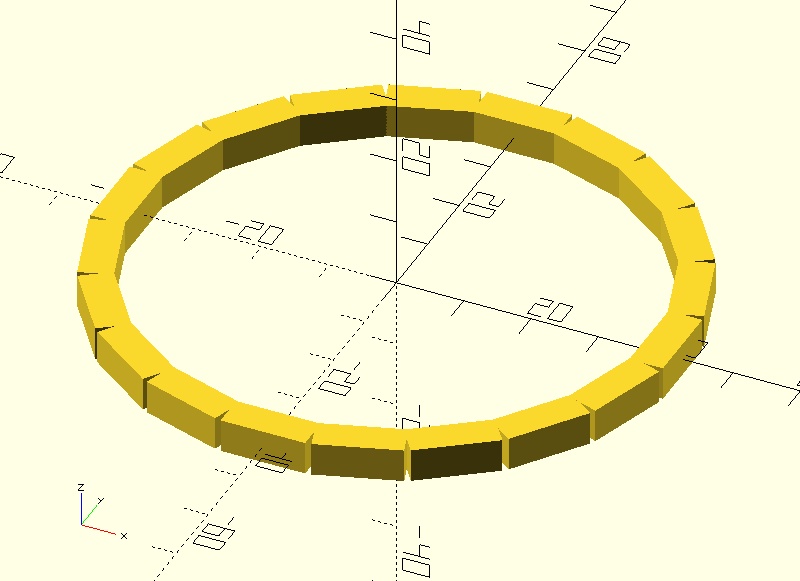
\includegraphics[width=.75\textwidth]{imagenes/piso}  
  \caption{Un piso de ladrillos.}\iftoggle{libro}{}{\vspace{128in}}
  \label{fig:piso}
\end{figure}

    
Los aplausos de Cecilia, al contemplar la figura \ref{fig:piso},
debieron escucharse hasta en la oficina de \director.


%%% Local Variables:
%%% mode: latex
%%% TeX-master: "../libro"
%%% End:
